\chapter{Trở thành giảng viên}

\diary{Hơi bị hay \href{https://techmaster.vn/khoa-hoc/25484/tro-thanh-giang-vien-gioi}{Ai cũng có thể trở thành giảng viên giỏi nếu} của anh Cường tại techmaster. Tưởng phải mua, hóa ra lại được set free. A hihi.}

\begin{itemize}
  \item Lên ý tưởng
  \item Chuẩn bị nội dung
  \item Code mẫu
  \item Xây dựng kịch bản
  \item Trình bày đơn giản, dễ hiểu
\end{itemize}

\section{Dạy và Học}

\subsection{Khác biệt giữa dạy online và offline}

Dạy online

\textbf{Ưu điểm}

\begin{enumerate}
  \item Khả năng mở rộng rất tốt
  \item Chi phí thấp
  \item Số lượng học viên không giới hạn
\end{enumerate}

\textbf{Nhược điểm}

\begin{itemize}
  \item Tỷ lệ bỏ học rất cao
  \item Tương tác chưa thực sự tốt
\end{itemize}

\subsection{Làm sao để giảm tỷ lệ bỏ học trực tuyến?}

\begin{itemize}
  \item Video ngắn < 10 phút
  \item Cấp chứng chỉ 70-90 USD lấy 1 chứng chỉ cho khóa học 4-6 tuần
  \item Chấm bài tập
  \item Facebook group kết nối giảng viên học viên
  \item Bài tập đủ dễ: chia nhỏ dự án khó ra
  \item Gamification: học như chơi
  \item Chịu khó email thông báo cho lớp
\end{itemize}

\subsection{Flip Learning}

Lớp học đảo ngược

Vấn đề học online

\begin{itemize}
  \item Bỏ học cao
  \item Tương tác face 2 face kém
  \item Thực hành không có, không kiểm soát
\end{itemize}

Vấn đề học offline

\begin{itemize}
  \item Chi phí cao
  \item Giao thông không thuận tiện
  \item Tuyển sinh khó
\end{itemize}

Flip Learning lớp học đảo ngược, kết hợp ưu điểm học trực tuyến và thực hành phòng lab.

- Khuyến khích học viên xem trước bài giảng video hướng dẫn giảng viên

- Đọc tìm hiểu thêm, trả lời trắc nghiệm qua Internet

- Tại buổi học, dành tối đa thời gian để \textbf{thực hành, hỏi đáp, hợp tác}

Khi đến lớp, học viên đã có kiến thức, biết rõ mình sẽ làm gì.

- Không thụ động, rèn tính tự học, tự đọc

- Không chống cằm nhìn giảng viên, không ghi chép

- Hỏi, làm, nói, giúp đỡ nhau

\textbf{Flip Learning:}

- Giảng viên phải chuẩn bị bài giảng

- Đến lớp trao đổi, hướng dẫn


\section{Sai lầm cố hữu của giảng viên}

1- Nghĩ ai cũng biết như mình.

Học viên 80\% từ nông thôn, 40\% thất nghiệp

Giảng viên dùng toàn từ chuyên ngành tiếng Anh mà không giải thích cặn kẽ

2- Nói nhiều, lý thuyết nhiều, ít có ví dụ, thí nghiệm minh họa. Học viên đã rất chán kiểu dạy ở đại học

3- Khô cứng: giải thích về kế thừa

4- Ba hoa, bốc phét như bán hàng đa cấp. Lesson online giới hạn 10 phút, học offline chỉ có 140 phút.

5- Dùng nhiều tính từ, đại ngôn: rất, cực.. mà không có con số.

6- Cẩu thả: không chuẩn bị kỹ slide, slide toàn chữ 12 trang.

7- Mã nguồn, dự án ví dụ vô duyên, khó hiểu

\begin{lstlisting}
  *
  **
  ***
  ****
  *****

  *     *
  *   *
  * *
  *
\end{lstlisting}

8- Chia nhỏ các bài tập


\section{Bước 1: Xây dựng khung giáo trình}

Các thông tin cơ bản của khóa học cần xác định khi thiết kế giáo trình cần có

\begin{itemize}
  \item Mục tiêu của khóa học
  \item Đối tượng của khóa học
  \item Thời lượng của khóa học
  \item Học xong khóa học này, học sinh có thể làm gì?
  \item Các gợi ý cho khóa học tiếp theo
\end{itemize}

\subsection{Xác định mục tiêu của khóa học}

Trong phần này, có thể tham khảo sách ebook, các khóa học được đánh giá cao trên Udemy, PluralSights, Lynda

Hãy xem một mục tiêu cực kỳ hấp dẫn của một \href{https://www.udemy.com/the-python-bible/}{khóa học về Python rất thành công trên udemy.com}

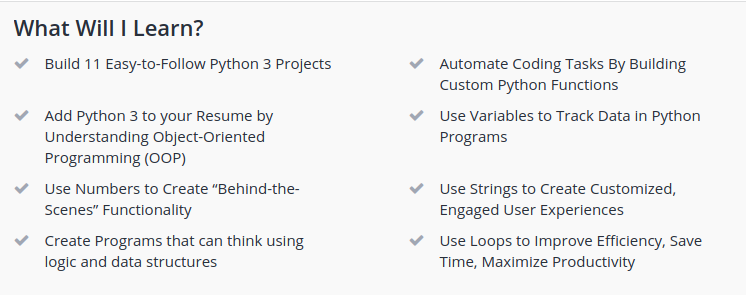
\includegraphics[width=\linewidth]{other/teaching/learning_objective.png}

Có lẽ điểm cộng quan trọng nhất trong khóa học này là \textbf{Xây dựng 11 dự án Python 3} - học xong khóa này học viên sẽ thực hiện được rất nhiều dự án

\subsection{Xác định đối tượng của khóa học}

Khi dạy một khóa học, điều quan trọng nhất để đạt được mục tiêu học tập đó là xác định đối tượng của khóa học là ai.

Có rất nhiều đối tượng tiềm năng

\begin{itemize}
  \item Sinh viên năm đầu: Họ rất cần kiến thức cơ bản, kinh nghiệm từ những người đi trước.
  \item Lập trình viên cần nâng cao kỹ năng: khi tiếp cận một công nghệ mới, lập trình viên muốn thông qua video có thể tiếp cận nhanh hơn với vấn đề
\end{itemize}

\textbf{Học viên Techmaster là ai?}

\begin{enumerate}
  \item Sinh viên CNTT năm đầu, cần thực hành: 30\%
  \item Người thất nghiệp: 40\%
  \item Lập trình cần nâng cao kỹ năng 30\%
  \item Hầu hết là từ nông thôn 70\%
  \item Thời gian có hạn, cần tìm việc ngay
\end{enumerate}

\textbf{Họ cần gì?}

\begin{enumerate}
  \item Bài giảng thực tế, có nhiều ví dụ sinh động
  \item Rất khác với ở trường đại học:
  \begin{itemize}
    \item Không phải thi
    \item Lý thuyết ít, thực hành nhiều, trừu tượng ít
    \item Ví dụ phải cool
    \item Có người hỗ trợ ngay
  \end{itemize}
  \item Trung tâm giới thiệu việc làm sau khi học
\end{enumerate}

\subsection{Thời lượng khóa học}

Thời lượng khóa học được tính bằng số lượng module, số lượng video, tổng thời lượng video.

Cần xác định với đối tượng học tập hiện tại, liệu họ có thể theo hết khóa học không?

\subsection{Khung giáo trình}

Mục tiêu của bước này là xây dựng khung giáo trình cho toàn bộ khóa học.

Các điều cần ghi nhớ

\begin{itemize}
  \item Top Down tốt hơn Bottom Up
\end{itemize}

Một công cụ hữu ích là MindMup, có thể dễ dàng tích hợp trong Google Drive

Người bình thường không thể nhớ quá 5 mục trong một buổi học:

\begin{itemize}
  \item Offline: 1 buổi dạy 1 chủ đề chia thành 4 minitask
  \item Online: 1 section gồm 4-5 video, mỗi video < 10 phút
\end{itemize}

Sử dụng MindMap

\textbf{Tài liệu tham khảo}

\begin{itemize}
  \item \href{https://techmaster.vn/khoa-hoc-online/25484/tro-thanh-giang-vien-gioi/3263/Xay-dung-khung-giao-trinh}{Xây dựng khung giáo trình, Trịnh Minh Cường}
\end{itemize}

\section{Bước 2: Xây dựng nội dung từng module}

\subsection{Thiết kế cấu trúc từng module}

Đầu và cuối mỗi module cần có một video overvew và summary.

Mỗi module nên có một sản phẩm cuối cùng

\textbf{Review 1:} Khoá \href{https://www.coursera.org/learn/machine-learning/home/welcome}{Machine Learning} của thầy Andrew Ng

\begin{itemize}
  \item Cả khóa học gồm 11 tuần
  \item 1 tuần có từ 2-3 section
  \item Mỗi section có từ 5-9 videos
  \item Mỗi section có từ 3-5 bài tập lập trình
\end{itemize}

\textbf{Review 2:} Khoá \href{https://techmaster.vn/khoa-hoc/25487/web-co-ban-html5-css3-va-javascript}{Web cơ bản HTML5, CSS3 và Javascript} của bạn Đặng Quang Huy

\begin{itemize}
  \item Cả khóa học có 79 bài học
  \item Có tất cả 19 module
  \item Mỗi module gồm 3-9 video
  \item Mỗi module sẽ có một bài tập
  \item Mỗi video từ 5-9 phút
\end{itemize}

\subsection{Thiết kế bài tập lập trình}

Bài tập lập trình cần \textbf{giống một trò chơi}, hay là \textbf{một ứng dụng thực tế}.

Học viên sẽ thấy phấn khích và thử thách khi thấy thành quả cuối cùng.

\section{Bước 3: Xây dựng một bài giảng pro}

\begin{tikzpicture}
  \node[draw] (analyze) at (0, 0) {kiến thức};
  \node[draw] (model) at (2, 0) {slide};
  \node[draw] (model) at (4, 0) {kịch bản};
  \node[draw] (model) at (0, -1) {code};
  \node[draw] (analyze) at (2, -1) {câu hỏi};
  \node[draw] (analyze) at (0, -2) {quay video};
  \node[draw] (analyze) at (2, -2) {nén video};
\end{tikzpicture}

\subsection{Thiết kế để học trực tuyến}

1- Một video < 10 phút. Tốt nhất 3 - 5 phút

2- Ví dụ là một dự án mẫu chạy được. Đơn giản tối đa

3- Học viên phấn khích khi thấy kết quả cuối cùng

4- Chia nhỏ task top-down:

+ Sản phẩm này làm gì?

+ Có chức năng gì? chỉ nên 1 hoặc 2

+ Màn hình chính

\subsection{Tính logic cấu trúc bài giảng}

Không nên:

- Tùy tiện theo ý thích hoặc kinh nghiệm cá nhân giảng viên
- Giập khuôn theo sách hoặc khóa học có sẵn
Hậu quả học nhiều, nhưng kỹ năng, kiến thức lộn xộn. Thà học ít mà dùng được nhiều, hiệu quả còn hơn

Nên:

- Thiết kế top down dùng Mindmap
- Các mẩu kiến thức có liên kết, sâu chuỗi

- Trước - Sau:
thủ tục -> hướng đối tượng -> design pattern
array -> dictionary -> linked list

SQL raw query -> Objection Relation Mapping

- Kế thừa: Cha - Con, Chị - Em

UIView > UIScollView > UITableView, UICollectionView

- Đối lập - so sánh:

Postgresql <> MongoDB, FireBase <> RethinkDB
Apple Push Notification <> Google Cloud Messaging

- Phân nhóm theo tiêu chí: Dễ học, dùng thường xuyên, học viên sướng. Sướng quyết định tất cả

Ví du:

- Lẻ tẻ, minh họa cụ thể từng cú pháp, API function. Học viên không thu hoạch được nhiều
- Một dự án kết hợp các bước sẽ thú vị hơn, dài hơn. Hay lúc đầu, buồn ngủ lúc sau.

\subsection{Tạo slide}

Slide ngắn gọn, xúc tích

Tự nhiên hôm nay (22/01/2018) lại đọc được bài \href{https://huynq.net/you-suck-at-powerpoint/}{You suck at PowerPoint}, thấy hay quá.

Sau đây là 10 lỗi thường gặp khi làm bài thuyết trình

\begin{enumerate}
  \item Quá nhiều chữ trong 1 slide.
  \item Màu chữ và màu nền không tương phản với nhau.
  \item Dùng clip art, word art.
  \item Hình ảnh sử dụng trong slide chất lượng kém, scale sai tỉ lệ.
  \item Sử dụng nhiều font chữ trong 1 slide.
  \item Lạm dụng quá nhiều hiệu ứng (animation/transition).
  \item Bài presentation không có cấu trúc.
  \item Slide không ăn nhập gì với nội dung trình bày.
  \item Không ghi rõ nguồn khi sử dụng tài liệu, hình ảnh của người khác.
  \item Ý thức của người làm slide
\end{enumerate}

\subsection{Viết kịch bản nói}

1- Viết chi tiết chính xác đến từng câu, rồi đọc lại
+ Nói chưa lưu loát > viết chi tiết
2- Liệt kê ý chính, vừa demo, vừa nói
+ Nói tốt + lười
+ Hậu kỳ phải cắt bỏ nhiều đoạn nói nhịu, ề à
Câu từ dài dòng, rườm ra, tỷ lệ tiếp thu càng thấp
Học trực tuyến, học viên dùng mắt đọc - xem là chính 70\%, nghe là phụ, 30\%. Video qua 5 phút gây buồn ngủ.

Nhắc kịch bản

- Không nên in ra giấy !
- Màn hình rộng Dell Utra, để mở cửa sổ nhắc kịch bản
- Mở rộng thêm 1 màn hình mới
- Gõ kịch bản ra iPad, dựng iPad lên thành màn hình phụ

\subsection{Đặt câu hỏi cho học viên}

Nếu không đặt câu hỏi:

\begin{itemize}
  \item Học viên thụ động, buồn ngủ, sớm rời bỏ khóa học
  \item Giảng viên không biết học viên có hiểu bài hay không?
\end{itemize}

\textbf{Đặt câu hỏi như thế nào?}

\begin{enumerate}
  \item Tránh Yes / No Question
  \item Câu hỏi để thức tỉnh khả năng suy nghĩ, động não
  \begin{enumerate}
    \item AJAX được ai phát minh ra? : chẳng có gì là quan trọng
    \item AJAX là viết tắt của cụm từ nào? : câu hỏi xem học viên có theo dõi video không?
    \item Một trang web hiển thị giá cổ phiếu cập nhật 15 giây một lần. Có 4000 khách hàng cùng truy cập, vậy có bao nhiêu AJAX gửi về máy chủ trong 1 giây? : đây là câu hỏi hay
  \end{enumerate}
  \item Câu hỏi ôn lại kiến thức
  \begin{itemize}
    \item Ý nghĩa của http verb GET, POST, PUT, DELETE là gì, khác nhau như thế nào? Câu hỏi rất rộng, không tốt
    \item Nhưng khi nào dùng POST và khi nào dùng PUT sẽ tập trung hơn và dễ tạo lựa chọn để trả lời.
    \item Sử dụng GET truyền id có thể thay thế DELETE được không? Tại sao không nên.
  \end{itemize}
  \item Hãy nhìn vào mắt học viên khi hỏi. (offline)
  \begin{itemize}
    \item Hỏi những học viên có dấu hiệu buồn ngủ
  \end{itemize}
\end{enumerate}

\section{Bước 4.1: Quay video}

\subsection{Chú ý khi quay video}

1- Camstasia 3 đã ra mắt

2- Ink2 Go

3- xScap

4- Terminal: font Roboto Mono for Powerline 18pt

5- Powerpoint 720p

\subsection{Các lỗi giảng viên thường mắc phải khi làm video}

1. Nói nhiều, thích ôm đồm nhiều thông tin trong một video > Độ dài tuyệt nhất là 3 phút

2. Chữ bé, các chi tiết khó nhìn khiến người dùng bị mỏi mắt > Thường sau 3-4 phút là khá mệt

3. Thiếu dòng title phút đầu tiên của video clip -> người dùng khó định hình ngày giảng viên muốn nói gì

4. Không điểm danh các mục nhỏ, nội dung trình bày trong video > Không biết sẽ đi về đâu

5. Không có điểm nhấn, phân cách giữa các mục nhỏ trong hướng dẫn > Mình đang ở mục mấy rồi nhỉ? Còn mấy mục nữa thì hết

6. Ít hình minh họa > Một hình ảnh dùng đúng hiệu quả hơn 1000 câu giải thích

7. Chỉ gõ lệnh nhưng ít khi nói mục đích để làm gì? Kết quả mong muốn là gì

8. Không giải thích các thuật ngữ mới

9. Chưa tính đến môi trường thực hành của học viên có thể khác so với giảng viên

\subsection{Đồ nghề tạo giáo trình trực tuyến}

1- Web Cam

+ Logitech C920 hoặc Xioami Camera loại 650,000VND.
+ Tỷ lệ bỏ lửng bài video giảm 30\% nếu học viên thấy mặt giảng viên.
+ Mặt giảng viên đẹp trai, hấp dẫn, hài hước càng tốt
+ Mở sẵn cửa sổ ứng dụng cần demo. Giảm tối đa thời gian chết

2- Camtasia

+ Camtasia Studio trên Windows có nhiều chức năng hơn bản Camtasia Mac
+ Phiên bản Camtasia Mac không nén được video định dạng H264 phải dùng FFmpeg để nén
+ Thu ở khung hình 1280 * 720 pixels. Trên Mac có công cụ xScope để căn kích thước màn hình thu

3- Phòng thu âm cần yên tĩnh

+ Đóng chặt cửa sổ, cửa phòng khi quay chấp nhật nóng trong 10 phút quay.
+ Bật chế noise remove trong Camtasia

4- Sublime Text
5- Ink2Go
6- Lucid Chart
7- Adobe Photoshop
8- Skitch
9- PowerPoint
10- Slides.com

\subsection{Kinh nghiệm khi quay video}

\textbf{Phòng cần yên tĩnh}: nên tắt quạt hay các thiết bị điện tử gây ồn. Tắt điện thoại tránh cuộc gọi đến khi đang ghi hình
Để micro xa bàn phím để không lẫn tiếng lạch cạch

Tuyệt đối không nên để background wallpaper lòe loẹt, học viên không chú ý vào demo của bạn mà xem background thì hiệu quả truyền đạt rất tệ. Tốt nhất để màn hình background là đen 100%

Tắt Skype, chat, loại bỏ các icon không cần thiết trên màn hình desktop

Nên dùng web camera Logitech C920 để xa mồm để không ghi tiếng thở hổn hển của giảng viên

Nên quay cả mặt giảng viên, nhưng cut crop để không quay background của phòng thu. Hãy để học viên tập trung vào bài giảng

Không sử dụng âm thanh nên có tiếng hát hoặc giai điệu nhanh, phức tạp khiến học viên không tập trung

Lưu ý rằng:

Học viên thích xem demo sinh động và đọc chữ trên màn hình rất nhanh, đừng nói quá dài dòng, phức tạp.

\subsection{Nén video chuẩn H.264}

Áp dụng đối với hệ điều hành Mac và Linux. Sau khi ghi hình ở độ phân giải 1280x720 pixels, và xuất ra video mp4. Nếu kích thước video tính theo Megabytes > 2 * số phút (Mb) thì video đó nén chưa tốt. Chúng ta cần phải nén video với chuẩn H264.

Các bước thực hiện

Vào web site này https://www.ffmpeg.org/ tải phần mềm ffmpeg về

Copy vào thư mục /usr/local/bin để có thể gọi ffmpeg ở mọi nơi
Tạo một bash script có tên v264 trong thư mục /usr/local/bin
cd /usr/local/bin
nano v264

Paste đoạn script này vào file v264

\begin{lstlisting}[language=bash]
  #!/bin/bash
  if [ -z "$1" ]; then
  echo "You must input video file name"
  exit
  fi
  if [ -f $1 ]; then
  output="$(echo $1 | sed 's/\.[^.]*$//')"
  ffmpeg -i $1 -c:a copy -x264-params crf=30 -b:a 64k "$output-264.mp4"
  else
  echo "File $1 does not exist"
  fi
\end{lstlisting}

Để file v264 thực thi được cần gõ lệnh để bổ xung quyền execution

\begin{lstlisting}[language=bash]
  chmod +x v264
\end{lstlisting}

Khi nén video gõ lệnh này

\begin{lstlisting}[language=bash]
  v264 yourvideo.mp4
\end{lstlisting}

\subsection{Upload video và tạo bài giảng}

Tạo một lesson như thế nào?

- Có một video dài < 10 phút

- Tối thiểu 3 câu hỏi quiz

- Nên bổ sung mã nguồn hoặc slide

\section{Bước 4.2: Thất bại khi thực hành}

Mọi lỗi sơ suất đều khiến giảng viên cực kỳ bối rối, áp lực
Mồ hôi toát ra như tắm, học viên xì xào, chán nản vì sốt ruột. Buổi học thất bại

Mọi demo cần chuẩn bị tập dượt, dù là chi tiết nhỏ nhất.

Thực hành tối thiểu 3 lần, ghi lại các bước thành Hand-On-Lab.
Ghi lại những lỗi giảng viên đã gặp phải:

- Cắm nhầm cực dương - âm tụ hóa

- Thiếu tụ lọc nhiễu

- Máy học viên có thể bị thiếu RAM, cấu hình sai

Giảng viên phát trước Hand-On-Lab cho học viên xem. Tạo câu hỏi quiz để đảm bảo học viên hiểu bài trước khi thực hành.

Đối với những bài thực hành khó, hãy yêu cầu học viên cài sẵn môi trường thực hành bởi:

1- Thời gian tải phần mềm ở lớp học có thể lâu
2- Tự học viên phát hiện lỗi khi cài phần mềm ở nhà
3- Học viên được làm quen trước với bài lab đơn giản

Đối với bài thực hành khó, hãy mạnh dạn chọn ra 1-2 học viên giỏi để chuẩn bị trước. Đây là đặc ân mà học viên giỏi sẽ thích thú và cố gắng tham gia.

\section{Bước 5: Học viên mất căn bản - Trả lời hỏi đáp}

\textbf{Question:} Trong một lớp học có quá nhiều học viên không có căn bản để học, nhưng lại có vài học viên giỏi, tiếp thu rất nhanh.

Phục vụ học viên mất căn bản hay phục vụ học viên giỏi?

\textbf{Trả lời:} Đừng chia thành 2 nhóm học viên giỏi và học viên kém. Nhóm giỏi sẽ tiếp tục đi nhanh hơn và nhóm kém sẽ bỏ cuộc.

Chia nhóm để ghép học viên giỏi và kém. Học viên giỏi sẽ giúp đỡ học viên kém.

Lớp 12 học viên chia thành 4 nhóm. Tạo ra cuộc thi đua nhỏ giữa các nhóm. Nếu có học viên bỏ học, sắp xếp lại nhóm.

\textbf{Question:} Trong một lớp học thực hành, nếu có nhiều câu hỏi ở mức độ khó khác nhau? Giảng viên chỉ được chọn trả lời một. Vậy chọn câu trả lời nào?

\textbf{Answer:} Hãy trả lời có khả năng hài lòng số đông học viên nhất.

Câu hỏi khó trả lời buổi sau, qua Facebook group của lớp

Câu hỏi ngoài lề không trả lời

Câu hỏi dễ, nhờ học viên khá trong lớp trả lời hộ

\section{Marketing}

Các hình thức marketing

1. Mạng xã hội: Facebook, forum
Phải boost quảng cáo. 500000 - 2000000 VND cho mỗi khóa học

2. SEO - Google Search

3. Qua hội thảo, meetup ~ hiệu quả thấp do số lượng người tham gia < 40 người

Conversation rate: số người mua hàng / số người tham quan

Nếu đến từ organic search CR = 1 / 200

Nếu qua chia sẻ bài viết mạng xã hội CR = 1 / 4000

Nếu qua giới thiệu, tư vấn người quen CR = 1 / 2

\subsection{Chia sẻ bài học trên Facebook}

Hoàn thành bài học

Một bài viết chia sẻ lên Facebook có ảnh sẽ được người dùng click vào cao gấp 2-3 lần bài viết không có ảnh.
Một bài viết có ảnh thumbnail có nút play xem video thì sẽ có số người dùng click vào cao hơn 1.3 lần so với ảnh thuần túy

Một khóa học online không giới thiệu qua Facebook, YouTube thì chắc chắn không có học viên dù giảng viên giỏi đến mấy

Bài giới thiệu trên facebook có nút play có lượt click lớn hơn nhiều so với không có nút play

\subsection{Sử dụng Photoshop}

Sử dụng Photoshop để làm poster cho khóa học